\documentclass{standalone}
\usepackage{tikz-network}
\begin{document}
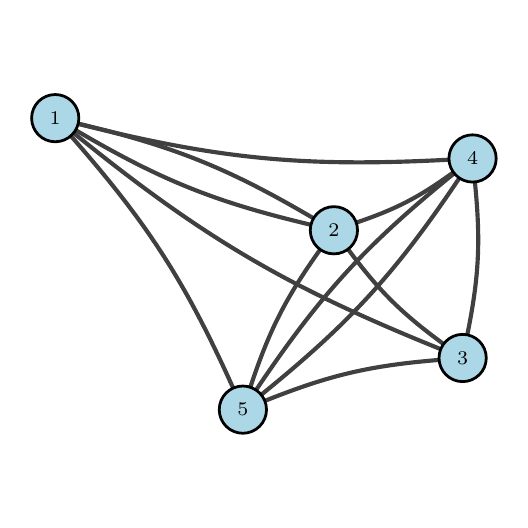
\begin{tikzpicture}
\clip (0,0) rectangle (6,6);
\Vertex[x=0.350,y=4.851,label=1,position=center]{1}
\Vertex[x=3.889,y=3.427,label=2,position=center]{2}
\Vertex[x=5.524,y=1.805,label=3,position=center]{3}
\Vertex[x=5.650,y=4.339,label=4,position=center]{4}
\Vertex[x=2.733,y=1.149,label=5,position=center]{5}
\Edge[,bend=-8.531](2)(1)
\Edge[,bend=-8.531](5)(1)
\Edge[,bend=-8.531](1)(2)
\Edge[,bend=-8.531](1)(3)
\Edge[,bend=-8.531](2)(3)
\Edge[,bend=-8.531](1)(4)
\Edge[,bend=-8.531](2)(4)
\Edge[,bend=-8.531](3)(4)
\Edge[,bend=-8.531](5)(4)
\Edge[,bend=-8.531](2)(5)
\Edge[,bend=-8.531](3)(5)
\Edge[,bend=-8.531](4)(5)
\end{tikzpicture}
\end{document}